\documentclass[runningheads]{llncs}

\usepackage[T1]{fontenc}
\usepackage{lmodern}
% T1 fonts will be used to generate the final print and online PDFs,
% so please use T1 fonts in your manuscript whenever possible.
% Other font encondings may result in incorrect characters.
%
\usepackage{graphicx}
% Used for displaying a sample figure. If possible, figure files should
% be included in EPS format.
%
% If you use the hyperref package, please uncomment the following two lines
% to display URLs in blue roman font according to Springer's eBook style:
%\usepackage{color}
%\renewcommand\UrlFont{\color{blue}\rmfamily}
%\urlstyle{rm}
%

\usepackage{prftree,tikz-cd}
\usepackage{amssymb,amsmath,cmll}
\let\proof\relax
\let\endproof\relax
\usepackage{amsthm}
\usepackage{lmodern}
\usepackage{adjustbox}
\usepackage[colorlinks=true,linkcolor=blue,urlcolor=teal]{hyperref}

% Agda formalization links
\newcommand{\agdaBaseUrl}{https://eapiova.github.io/nuclear}
\newcommand{\agdalink}[1]{\href{\agdaBaseUrl/#1}{\raisebox{-0.1em}{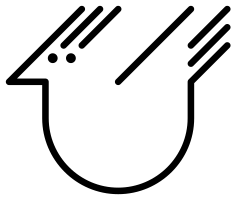
\includegraphics[height=0.9em]{agda-bird}}}}

%\renewcommand{\L}{\mathbf{L}}
\newcommand{\FL}{\mathbf{FL}}
\newcommand{\InFL}{\mathbf{InFL}}
\newcommand{\FLe}{\mathbf{FL_e}}
\newcommand{\InFLe}{\mathbf{InFL_e}}
\newcommand{\Min}{\mathbf{Min}}
\newcommand{\Cl}{\mathbf{Cla}}
\newcommand{\Gl}{\mathbf{Gli}}
\newcommand{\Int}{\mathbf{Int}}
\newcommand{\Neg}{\mathbf{Neg}}

\DeclareMathOperator{\Glivenko}{G}
\DeclareMathOperator{\Kleisli}{K}
\DeclareMathOperator{\Maximal}{M}
\DeclareMathOperator{\FO}{FO}
\DeclareMathOperator{\Inf}{Inf}
\DeclareMathOperator{\Mod}{Mod}
\DeclareMathOperator{\Lin}{Lin}

\begin{document}
%
\title{Glivenko's theorem underneath structure}
%
%\titlerunning{Abbreviated paper title}
% If the paper title is too long for the running head, you can set
% an abbreviated paper title here
%
\author{
    Riccardo Borsetto\inst{1}\orcidID{0009-0001-4751-1516} \and
    Giulio Fellin\inst{1}\orcidID{0000-0002-3179-7521} \and
    Tarmo Uustalu\inst{2,3}\orcidID{0000-0002-1297-0579} \and
    Cheng-Syuan Wan\inst{3}\orcidID{0000-0003-2053-1688}}
%
\authorrunning{R. Borsetto et al.}
% First names are abbreviated in the running head.
% If there are more than two authors, 'et al.' is used.
%
\institute{Università degli Studi di Verona, Italy\\
    \email{\{riccardo.borsetto,giulio.fellin\}@univr.it} \and
    Reykjavik University, Iceland\\
    \email{tarmo@ru.is}\and
    Tallinn University of Technology, Estonia\\
    \email{\{tarmo,cswan\}@cs.ioc.ee}}
%
\maketitle              % typeset the header of the contribution
%
\begin{abstract}
    Glivenko's theorem has been studied in an abstract setting, where double negation is replaced by arbitrary nuclei, and classical and intuitionistic propositional logics are generalised to abstract entailment relations. This paper extends that framework to substructural logics, focusing on cases where structural rules such as weakening, contraction, and exchange are restricted. We apply our findings to Full Lambek logic and its extensions, in order to derive a few Glivenko-style theorems. All results are developed within an intuitionistic meta-theory, allowing a computational interpretation and direct formalisation in Agda.
    
    \keywords{Glivenko's theorem \and
        Full Lambek calculus \and
        Substructural logics \and
        Nuclei \and
        Structural proof theory \and
        Agda
    }
\end{abstract}
%
%
%
\section{Introduction}

Glivenko's theorem is one of the earliest and most influential results relating classical and intuitionistic logic. Established in the setting of propositional logic, it states that the classical provability of a formula implies the intuitionistic provability of its double negation \cite{gliv28,gliv29}:
\[
\Cl \vdash U \rhd a \iff \Int \vdash U \rhd \neg\neg a,
\]
where $\Cl$ and $\Int$ denote classical and intuitionistic propositional logic, respectively.

Results of this kind are often referred to as \emph{conservation} or \emph{translation} results between logical systems. Their importance lies in the fact that they allow classical reasoning to be studied within a constructive framework. Rather than treating classical and intuitionistic mathematics as entirely separate enterprises, such results make it possible to identify which parts of classical reasoning can be faithfully interpreted in constructive terms. This is particularly significant because intuitionistic proofs often admit computational interpretations---for instance through the Curry--Howard correspondence---so that translating classical arguments into intuitionistic ones may reveal their underlying computational content.

Over time, a number of generalisations of Glivenko's theorem have been investigated, often by replacing $\Int$ with weaker logics. In 1968, Segerberg \cite{Segerberg1968-SEGPLR} introduced the \emph{Glivenko logic}~$\Gl$, defined as Johansson's minimal logic extended by the double negation of \emph{ex falso quodlibet sequitur}, namely $\neg\neg(\bot \to a)$. In the same paper, he claimed---without proof or citation---a characterisation result that was later formally established by Odintsov \cite{Odintsov02,Odintsov2004-ODINEO-2}: the Glivenko logic is the smallest logic for which Glivenko's theorem holds. More precisely, for any logic $\mathbf{L}$ such that $\Min \subseteq \mathbf{L} \subseteq \Cl$, the following are equivalent:
\begin{enumerate}
    \item $\Cl \vdash U \rhd a$ if and only if $\mathbf{L} \vdash U \rhd \neg\neg a$;
    \item $\mathbf{L}$ is an extension of $\Gl$, i.e. it satisfies the condition $\mathbf{L}\vdash\neg\neg(\bot \to a)$.
\end{enumerate}

Extensions of this result to substructural logics were developed by Cignoli and Torrens \cite{Cignoli2003-CIGHBF,CignoliTorrens}, and by Galatos and Ono \cite{GO:glitsl,ResLat}. Subsequently, Ono \cite{ono:gli} established an analogue of Segerberg's characterisation for the Full Lambek logic with exchange, $\FLe$---that is, intuitionistic linear logic without exponentials---and its \emph{involutive} extension $\InFLe$, obtained by adding the stability axiom $\neg\neg a \rhd a$ to $\FLe$. Ono's theorem states that for any logic $\mathbf{L}$ such that $\FLe \subseteq \mathbf{L} \subseteq \InFLe$, the following conditions are equivalent:
\begin{enumerate}
    \item $\InFLe \vdash U \rhd a$ if and only if $\mathbf{L} \vdash U \rhd \neg\neg a$;
    \item The following conditions are satisfied:
    \begin{itemize}
        \item $\mathbf{L} \vdash \neg(a \wedge b) \rhd \neg(\neg\neg a \wedge \neg\neg b)$;
        \item $\mathbf{L} \vdash \neg(a \to b) \rhd \neg(\neg\neg a \to \neg\neg b)$.
    \end{itemize}
\end{enumerate}

Double negation in intuitionistic logic is a specific instance of a \emph{nucleus} \cite{aczel:aspects,hayk:more,joh:sto,negri:cont,rosen,simm:frame,simm:cur}---also referred to as a strong monad \cite{kock:sdg} or lax modality \cite{aczel_2001}---defined as a map $j$ on formulae satisfying the following \cite{van:kuroda}:
\[
(a \to j(b)) \lhd\!\!\rhd (j(a) \to j(b)).
\]

Fellin and Schuster \cite{fel:nuclei,fel:cat} generalised Glivenko's theorem by replacing double negation with an arbitrary nucleus, thereby moving from syntactic provability in a particular calculus to the more general setting of inductively generated abstract consequence relations, and extending the framework from propositional formulas to arbitrary objects. They provided precise criteria under which a classical-style generalisation yields a conservative extension of its intuitionistic counterpart via a nucleus.

The present work extends the framework of \cite{fel:nuclei,fel:cat} to entailment relations that may lack structural rules such as weakening, contraction, and exchange \cite{PAOLI,restall:sub}. In the traditional structural setting, the presence of exchange together with implication ensures that $j$ remains a nucleus over all inductive extensions of $\mathbf{L}$. In the more general substructural context, however, this property no longer holds automatically. As a consequence, the assumption that $j$ is a nucleus over the initial relation cannot in general be propagated to its extensions, and the role of the nucleus must be analysed more carefully. This makes it possible, in particular, to dispense with the initial nucleus assumption that is typically required in the structural case.

Another important feature of the main theorem in the present paper is that it further investigates the inclusion relationships between the various extensions induced by nuclei, thereby generalising and expanding characterisations that have appeared in the literature.

The paper is organised as follows. Section~\ref{entrel} introduces substructural entailment relations and establishes the abstract Conservation theorem (Theorem~\ref{thm-conservation}). Section~\ref{sec-nuclei} analyses left, right and bi-nuclei. Section~\ref{sec-FL} specialises the framework to the substructural \emph{Full Lambek logic}~$\FL$ and its extensions \cite{Lambek1958TheMO,Lambek1961OnTC,Lambek1995SomeLM}, where we prove the Conservation theorem for~$\FL$ (Theorem~\ref{thm-FL}); from it we derive Corollary~\ref{cor-glivenko}, which, by instantiating the Glivenko nucleus~$\neg\neg$ \cite{van:kuroda,esca:peirce}, recovers the substructural results of Ono and of Galatos--Ono \cite{GO:glitsl,ResLat,ono:gli}, and Corollary~\ref{cor-open} for the \emph{open nucleus}, which remains meaningful in the noncommutative setting. Section~\ref{sec-future} outlines directions for future work.

All the results in this paper are developed within an intuitionistic meta-theory. Working constructively at the meta-level ensures that the arguments themselves admit a computational interpretation and avoids relying on classical principles that would be incompatible with the constructive perspective underlying much of the work. An additional benefit of this approach is that the main constructions and proofs can be directly formalised in a proof assistant. In particular, we have implemented the results in Agda~\cite{norell:agda}\footnote{The formalisation is built on top of the \texttt{agda/cubical} library~\cite{vezzosi:cubicalagda}.}, providing a machine-checked formalisation of the main definitions and theorems. The source code is available at~\cite{nuclear:agda}. This formalisation is partially based on the Agda development by Altenkirch~\cite{altenkirch:nuclear}. Throughout the paper, the symbol \agdalink{Substructural.Everything.html} next to a definition or theorem header is a clickable link to the corresponding formalised statement in the HTML rendering of the Agda source.

\section{Substructural entailment relations and conservation}
\label{entrel}

Let $S$ be a set and $S^*$ be the set of finite lists of elements of $S$.
Given $\mathbf{L}\subseteq S^*\times S$, we write
$ \mathbf{L}\vdash U\rhd b $
in place of $(U,b)\in\mathbf{L}$. 
The expression ``$U\rhd b$'' is called \emph{sequent}.

A \emph{(single-conclusion) substructural entailment relation} is a relation $\mathbf{L}\subseteq S^*\times S$
such that 
\begin{align*}
    \prftree[r]{Refl}{a\rhd a} &&
    \prftree[r]{Trans}{U\rhd a}{}{V_1,a,V_2\rhd b}{V_1,U,V_2\rhd b}
\end{align*}
These two are the \emph{structural rules} of \emph{reflexivity} and \emph{transitivity}, respectively.

Optional structural rules include \emph{commutativity} (or \emph{exchange}), \emph{monotonicity} (or \emph{weakening}) and \emph{contraction}:
\begin{align*}
    \prftree[r]{Comm}{U_1,a_1,a_2,U_2\rhd b}{U_1,a_2,a_1,U_2\rhd b} &&
    \prftree[r]{Mono}{U_1,U_2\rhd b}{U_1,a,U_2\rhd b} &&
    \prftree[r]{Contr}{U_1,a,a,U_2\rhd b}{U_1,a,U_2\rhd b}
\end{align*}

Quite often an entailment relation $\mathbf{L}$ is inductively generated from a given set $\mathcal{R}$ of rules by closing up with respect to the structural rules above. These \emph{non-structural rules} have the  form
\begin{align*}
    \prftree[r]{\textnormal{$r$}}{U_1\rhd b_1}{...}{U_n\rhd b_n}{U\rhd b}
    &&\textnormal{or, more compactly,}&&
    \prftree[r]{\textnormal{$r$}}{\{U_i\rhd b_i\colon 1\leq i\leq n\}}{U\rhd b}
\end{align*}
We call \emph{axioms} the rules that are premissless, i.e. have the form
\begin{align*}
    \prftree[r]{\textnormal{$r$}}{U\rhd b}
\end{align*}
If $\mathbf{L}$ is inductively generated by a set $\mathcal{R}$ of rules, we write $\mathbf{L}=\langle \mathcal{R}\rangle$.

An inductively generated entailment relation $\rhd$ can have multiple generating rule sets $\mathcal{R}$. Despite this, it is common to refer to an inductively generated entailment relation $\rhd$ without specifying a set of generating rules $\mathcal{R}$, unless statements about $\rhd$ depend on $\mathcal{R}$.

By an \emph{extension} ${\mathbf{L}'}$ of an entailment relation ${\mathbf{L}}$ we mean in general 
an entailment relation such that 
${\mathbf{L}}\subseteq{\mathbf{L}'}$.
We also say that $\mathbf{L}'=\langle\mathcal{R},\mathcal{R}'\rangle$ is an \emph{inductive extension} of $\mathbf{L}=\langle\mathcal{R}\rangle$, and we call $\mathcal{R}'$ the set of \emph{additional rules}. 

\begin{definition}[\agdalink{Substructural.Core.Nucleus.html}]
    Consider the following rules:
    \begin{align*}
        \prftree[r]{\textnormal{L$j$}}{U,a,V\rhd j(b)}{U,j(a),V\rhd j(b)}
        &&
        \prftree[r]{\textnormal{R$j$}}{U\rhd b}{U\rhd j(b)}
    \end{align*}
    Given a set $S$ endowed with an entailment relation $\mathbf{L}$,
    we say that a function $j\colon S\to S$ is 
    \begin{itemize}
        \item \emph{expansive (over $\mathbf{L}$)} if \textnormal{R$j$} holds
        in $\mathbf{L}$;
        \item a \emph{bi-nucleus (over $\mathbf{L}$)} if both \textnormal{L$j$} and \textnormal{R$j$} hold in $\mathbf{L}$.
    \end{itemize}
\end{definition}

\begin{definition}[\agdalink{Substructural.Core.Nucleus.html\#rj}]
    Let $j\colon S\to S$.
    Given a rule $r$, its \emph{$j$-version} $r_j$ is obtained by putting $j$ in front of every succedent:
    \[
        \prftree[r]{\textnormal{$r$}}{\{U_i\rhd b_i\colon i\in I\}}{U\rhd b}
        \quad\rightsquigarrow\quad
        \prftree[r]{\textnormal{$r_j$}}{\{U_i\rhd j(b_i)\colon i\in I\}}{U\rhd j(b)}
    \]
    We write $\mathcal{R}_j$ for $\{r_j\colon r\in\mathcal{R}\}$.
    Given a rule $r$ that is admissible in $\mathbf{L}$, we say that $r$ \emph{survives after $j$ (over $\mathbf{L}$)} if $r_j$ is admissible in $\mathbf{L}$.
    %
    We also define the \emph{stability axiom} for $j$:
    \begin{align*}
        \prftree[r]{\textnormal{$j$-stab}}{j(a)\rhd a}
    \end{align*}
\end{definition}
Stability for $j$ is a abstract version of the \emph{double negation elimination} axiom, which defines classical logic.

\begin{remark}[\agdalink{Substructural.Core.Conservation.html\#remark1}]\label{lem-reflj}\
    We observe the following:
    \begin{enumerate}
        \item \label{item-reflj}
        \textnormal{R$j$} and \textnormal{Refl$_j$} are equivalent in $\mathbf{L}$.
        \item \label{item-transj}
        \textnormal{L$j$} and \textnormal{Trans$_j$} are equivalent in $\mathbf{L}$.
        \item \label{item-jstab}
        \textnormal{$j$-stab} and the following are equivalent in $\mathbf{L}$
        \[ \prftree[r]{\textnormal{L$j^+$}}{U,a,V\rhd b}{U,j(a),V\rhd b} \]
        In particular, \textnormal{$j$-stab} entails \textnormal{L$j$}.
    \end{enumerate}
\end{remark}

\begin{definition}[\agdalink{Substructural.Core.Extensions.html}]
    Given an inductively generated entailment relation $\mathbf{L}=\langle \mathcal{R}\rangle$ and an expansive function $j$ on $\mathbf{L}$, we define the following extensions:
    \begin{enumerate}
        \item the \emph{Kleisli $j$-extension} $\Kleisli_j(\mathbf{L})$ of $\mathbf{L}$ by
        \begin{align*}
            \Kleisli_j(\mathbf{L}):=\{ (U, a)\colon \mathbf{L}\vdash U\rhd j(a)\},
        \end{align*}
        \item the \emph{Glivenko $j$-extension} $\Glivenko_j(\mathbf{L})$ of $\mathbf{L}$ as
        \begin{align*}
            \Glivenko_j(\mathbf{L}):=\langle\mathcal{R},\mathcal{R}_j,\{\textnormal{L$j$}\}\rangle,
        \end{align*}
        \item the \emph{Kleisli-stable $j$-extension} $\Maximal_j(\mathbf{L})$ of $\mathbf{L}$ as
        %\footnote{The notation here is adapted from \cite[\S 8.2]{ResLat}. The ``M'' stands for ``maximum,'' as $\Maximal_j(\mathbf{L})$ is the greatest extension $\mathbf{L}'$ of $\mathbf{L}$ such that $\Kleisli_j(\mathbf{L}')\subseteq\Maximal_j(\mathbf{L})$. See Theorem \ref{thm-conservation}.\ref{cons-3}, cf. \cite[Theorem 8.7]{ResLat}.}
        \begin{align*}
            \Maximal_j(\mathbf{L}):=\langle\mathcal{R},\{\textnormal{$j$-stab}\}\rangle.
        \end{align*}
    \end{enumerate}
\end{definition}
Intuitively, the Glivenko $j$-extension corresponds to an abstract version of the Glivenko logic, and the Kleisli-stable $j$-extension corresponds to an abstract version of classical logic.
Although the definitions of $\Glivenko_j(\mathbf{L})$ and $\Maximal_j(\mathbf{L})$ are given in terms of the generating set $\mathcal{R}$ rather than $\mathbf{L}$ itself, we always consider $\mathcal{R}$ fixed as the generator of $\mathbf{L}$.

\begin{remark}
    Clearly, $j$ is a bi-nucleus over $\Glivenko_j(\mathbf{L})$.
\end{remark}

\begin{proposition}[\agdalink{Substructural.Core.Conservation.html\#proposition1}]\label{prop-ext}\
    Let $S$ be a set endowed with an inductively generated entailment relation $\mathbf{L}=\langle \mathcal{R}\rangle$, and let $j$ be expansive over $\mathbf{L}$.
    Then the following inclusions hold:
    \begin{center}
        \begin{tikzcd}
            \mathbf{L}\arrow[hook,r]\arrow[hook,d]
            &\Glivenko_j(\mathbf{L})\arrow[hook,d]
            \\
            \Kleisli_j(\mathbf{L})\arrow[hook,r]
            &\Maximal_j(\mathbf{L})
        \end{tikzcd}
    \end{center}
\end{proposition}
\begin{proof}\
    \begin{itemize}
        \item $\mathbf{L}\subseteq\Kleisli_j(\mathbf{L})$ is nothing but R$j$.
        \item $\mathbf{L}\subseteq\Glivenko_j(\mathbf{L})$ follows from the definition of $\Glivenko_j(\mathbf{L})$.
        \item $\Glivenko_j(\mathbf{L})\subseteq\Maximal_j(\mathbf{L})$: It suffices to show that the latter admits all rules in the inductive definition of the former. Rule L$j$ is guaranteed by $j$-stab, see Remark \ref{lem-reflj}. The only non-trivial remaining cases are the $r_j$ where $r\in\mathcal{R}$. Let us consider 
        \[
        \prftree[r]{\textnormal{$r$}}{\{U_i\rhd b_i\colon i\in I\}}{U\rhd b}
        \quad\rightsquigarrow\quad
        \prftree[r]{\textnormal{$r_j$}}{\{U_i\rhd j(b_i)\colon i\in I\}}{U\rhd j(b)}
        \]
        We have the following in $\Maximal_j(\mathbf{L})$:
        \[
        \prftree[r]{\textnormal{R$_j$}}{
            \prftree[r]{\textnormal{$r$}}{...}{
                \prftree[r]{Trans}{
                    {U_i\rhd j(b_i)}
                }{
                    \prftree[r]{\textnormal{$j$-stab}}{j(b_i)\rhd b_i}
                }{ U_i\rhd b_i}
            }{\prfassumption{...}}{ U\rhd b}
        }{ U\rhd j(b)}
        \]
        \item $\Kleisli_j(\mathbf{L})\subseteq\Maximal_j(\mathbf{L})$:
        \[
        \prftree[r]{Trans}{
            \prftree[r]{defn}{
                \prftree[r]{defn}{
                    {\Kleisli_j(\mathbf{L})\vdash U\rhd b}
                }{\mathbf{L}\vdash U\rhd j(b)}
            }{\Maximal_j(\mathbf{L})\vdash U\rhd j(b)}
        }{
            \prftree[r]{\textnormal{$j$-stab}}{\Maximal_j(\mathbf{L})\vdash j(b)\rhd b}
        }{\Maximal_j(\mathbf{L})\vdash U\rhd b}
        \qedhere
        \]
    \end{itemize}
\end{proof}

\begin{theorem}[Conservation \agdalink{Substructural.Core.Conservation.html\#theorem1}]\label{thm-conservation}
    Let $\mathbf{L}=\langle \mathcal{R}\rangle$, let $\mathbf{L}'=\langle\mathcal{R},\mathcal{R}'\rangle$, and let $j$ be expansive over $\mathbf{L}$.
    Then:
    \begin{align}
        \Kleisli_j(\mathbf{L}')\supseteq\mathbf{L}'&
        \label{cons-1}
        \\
        \Kleisli_j(\mathbf{L}')\subseteq\mathbf{L}'&\iff\mathbf{L}'\supseteq\Maximal_j(\mathbf{L})
        \label{cons-2}
        \\
        \Kleisli_j(\mathbf{L}')\subseteq\Maximal_j(\mathbf{L})&\iff\mathbf{L}'\subseteq\Maximal_j(\mathbf{L})
        \label{cons-3}
        \\
        \Kleisli_j(\mathbf{L}')\supseteq\Maximal_j(\mathbf{L})&\iff\mathbf{L}'\supseteq\Glivenko_j(\mathbf{L})
        \label{cons-4}
    \end{align}
\end{theorem}

\begin{proof}\
    \begin{enumerate}
        \item[(\ref{cons-1})] A particular case of Proposition \ref{prop-ext}.
        \item[(\ref{cons-2})] If $\mathbf{L}'\supseteq\Maximal_j(\mathbf{L})$, then in particular $\mathbf{L}'\vdash j(a)\rhd a$. Let us suppose $\Kleisli_j(\mathbf{L}')\vdash U\rhd a$, i.e. $\mathbf{L}'\vdash U\rhd j(a)$. Then by Trans we conclude $\mathbf{L}'\vdash U\rhd a$. We have shown $\Kleisli_j(\mathbf{L}')\subseteq\mathbf{L}'$.
        
        Now suppose that $\Kleisli_j(\mathbf{L}')\subseteq\mathbf{L}'$. From $\mathbf{L}'\vdash j(a)\rhd j(a)$, i.e. $\Kleisli_j(\mathbf{L}')\vdash j(a)\rhd a$, we get $\mathbf{L}'\vdash j(a)\rhd a$ by assumption.
        This means that $j$-stab holds in $\mathbf{L}'$,
        which suffices for $\mathbf{L}'\supseteq\Maximal_j(\mathbf{L})$.
        \item[(\ref{cons-3})] The direction ``$\Rightarrow$'' easily follows from $\mathbf{L}'\subseteq\Kleisli_j(\mathbf{L}')$ (Proposition \ref{prop-ext}).
        
        Now suppose that $\mathbf{L}'\subseteq\Maximal_j(\mathbf{L})$.
        Since $\mathbf{L}\subseteq\mathbf{L}'$, we have $\Maximal_j(\mathbf{L})\subseteq\Maximal_j(\mathbf{L}')$.
        On the other hand, as stability and all the rules of $\mathbf{L}'$ are admissible in $\Maximal_j(\mathbf{L})$, we also have $\Maximal_j(\mathbf{L}')\subseteq\Maximal_j(\mathbf{L})$.
        Therefore $\Maximal_j(\mathbf{L})=\Maximal_j(\mathbf{L}')$. From this and $\Kleisli_j(\mathbf{L}')\subseteq\Maximal_j(\mathbf{L}')$ (Proposition \ref{prop-ext}), we conclude $\Kleisli_j(\mathbf{L}')\subseteq\Maximal_j(\mathbf{L})$.
        \item[(\ref{cons-4})] Assume $\mathbf{L}'\supseteq\Glivenko_j(\mathbf{L})$, and suppose $\Maximal_j(\mathbf{L})\vdash U\rhd a$. We prove that $\Glivenko_j(\mathbf{L})\vdash U\rhd ja$ by induction on the last rule $r$ used in the derivation of $\Maximal_j(\mathbf{L})\vdash U\rhd a$. The case in which $r\in\mathcal{R}\cup\{\text{Trans},\text{Refl}\}$ is converted in $\Glivenko_j(\mathbf{L})$ to an application of the rule $r_j$, while the case in which $r$ is $j$-stab is converted to an instance of Refl. So we have proved $\Glivenko_j(\mathbf{L})\vdash U\rhd ja$, which by hypothesis implies $\mathbf{L}'\vdash U\rhd ja$, i.e. $\Kleisli_j(\mathbf{L}')\vdash U\rhd a$ as desired.
        
        Assume $\Kleisli_j(\mathbf{L}')\supseteq\Maximal_j(\mathbf{L})$. 
        Suppose that $\Glivenko_j(\mathbf{L})\vdash U\rhd a$. We prove $\mathbf{L}'\vdash U\rhd a$ by induction on the last rule used in the derivation of $\Glivenko_j(\mathbf{L})\vdash U\rhd a$.
        \begin{enumerate}
            \item Case $r\in \mathcal{R}$:
            We have
            \[
            \prftree[r]{\textnormal{$r$}}{\Glivenko_j(\mathbf{L})\vdash U_1\rhd a_1}{...}{\Glivenko_j(\mathbf{L})\vdash U_n\rhd a_n}{\Glivenko_j(\mathbf{L})\vdash U\rhd a}
            \]
            which leads to
            \[
            \prftree[r]{\textnormal{$r$}}{
                \prftree[r]{ind. hp.}{\Glivenko_j(\mathbf{L})\vdash U_1\rhd a_1}{\mathbf{L}'\vdash U_1\rhd a_1}
            }{...}{
                \prftree[r]{ind. hp.}{\Glivenko_j(\mathbf{L})\vdash U_n\rhd a_n}{\mathbf{L}'\vdash U_n\rhd a_n}
            }{\mathbf{L}'\vdash U\rhd a}
            \]
            \item Case $r=\textnormal{L$j$}$ or $r_j$ (where $r\in \mathcal{R}$): We have $a = j(b)$ for some $b \in S$, and hence we can write $\Glivenko_j(\mathbf{L}) \vdash U \rhd j(b)$. Since $\Glivenko_j(\mathbf{L}) \subseteq \Maximal_j(\mathbf{L}) \subseteq \Kleisli_j(\mathbf{L}')$, it follows that $\Kleisli_j(\mathbf{L}') \vdash U \rhd j(b)$. By the definition of $\Kleisli_j(\mathbf{L}')$, this is equivalent to $\mathbf{L}' \vdash U \rhd j(j(b))$. 
            On the other hand, we observe that $\Maximal_j(\mathbf{L})\vdash j(j(b))\rhd b$ by applying L$j^+$ twice. Then $\Maximal_j(\mathbf{L})\subseteq\Kleisli_j(\mathbf{L}')$ implies $\Kleisli_j(\mathbf{L}')\vdash j(j(b))\rhd b$, which is nothing but $\mathbf{L}'\vdash j(j(b))\rhd j(b)$.
            By an application of transitivity between $\mathbf{L}' \vdash U \rhd j(j(b))$ and $\mathbf{L}'\vdash j(j(b))\rhd j(b)$, we conclude $\mathbf{L}' \vdash U \rhd j(b)$.
            \qedhere
        \end{enumerate}
    \end{enumerate}
\end{proof}

In particular, we observe that $\Maximal_j(\mathbf{L})$ is the smallest extension $\mathbf{L}'$ of $\mathbf{L}$ for which $\Kleisli_j(\mathbf{L}') = \mathbf{L}'$. We also notice that $\Kleisli_j(\mathbf{L}') = \Kleisli_j\Maximal_j(\mathbf{L})$ if and only if $\mathbf{L}'$ is intermediate between $\Glivenko_j(\mathbf{L})$ and $\Maximal_j(\mathbf{L})$.
Visually, we can summarise some of the main cases as follows:
\vspace{-10pt}
\begin{center}
\begin{adjustbox}{max width=\textwidth}
    \begin{tikzcd}
        \mathbf{L}\arrow[hook,r]\arrow[hook,d]
        &\mathbf{L}_1\arrow[hook,r]\arrow[hook,d]
        &\Glivenko_j(\mathbf{L})\arrow[hook,r]\arrow[hook,d]
        &\mathbf{L}_2\arrow[hook,r]\arrow[hook,d]
        &\Maximal_j(\mathbf{L})\arrow[hook,r]\arrow[equal,d]
        &\mathbf{L}_3\arrow[equal,d]
        \\
        \Kleisli_j(\mathbf{L})\arrow[hook,r]
        &\Kleisli_j(\mathbf{L}_1)\arrow[hook,r]
        &\Kleisli_j\Glivenko_j(\mathbf{L})\arrow[equal,r]
        &\Kleisli_j(\mathbf{L}_2)\arrow[equal,r]
        &\Kleisli_j\Maximal_j(\mathbf{L})\arrow[hook,r]
        &\Kleisli_j(\mathbf{L}_3)
    \end{tikzcd}
\end{adjustbox}
\end{center}

\section{Left and right nuclei}\label{sec-nuclei}

In the previous section, we introduced the notion of \emph{bi-nucleus}, which allows rule \textnormal{L$j$} to be applied to any element on the left-hand side of the sequent. This is sufficient for the main conservation theorem. However, in concrete cases many functions $j$ satisfy only a weaker version of the rule \textnormal{L$j$}, which can be applied only to elements occurring in specific positions. For this reason, we introduce the notions of \emph{left nucleus} and \emph{right nucleus}.

\begin{definition}[\agdalink{Substructural.Core.Nucleus.html}]
    Consider the following rules:
    \begin{align*}
        \prftree[r]{\textnormal{L$j_\textnormal{left}$}}{U,a\rhd j(b)}{U,j(a)\rhd j(b)}
        &&
        \prftree[r]{\textnormal{L$j_\textnormal{right}$}}{a,U\rhd j(b)}{j(a),U\rhd j(b)}
    \end{align*}
    Given a set $S$ endowed with an entailment relation $\mathbf{L}$,
    we say that an expansive function $j\colon S\to S$ is 
    \begin{itemize}
        \item a \emph{right nucleus (over $\mathbf{L}$)} if \textnormal{L$j_\textnormal{right}$} holds in $\mathbf{L}$;
        \item a \emph{left nucleus (over $\mathbf{L}$)} if \textnormal{L$j_\textnormal{left}$} holds in $\mathbf{L}$.
    \end{itemize}
\end{definition}

\begin{remark}[\agdalink{Substructural.Core.Conservation.html\#remark2}]\
    \begin{enumerate}
        \item Every bi-nucleus is both a left and right nucleus.
        \item If Comm is admissible in $\mathbf{L}$, then the definitions of right, left and bi-nucleus coincide.
    \end{enumerate}
\end{remark}

\begin{remark}[\agdalink{Substructural.Core.Conservation.html\#remark3}]\label{lem-K-Trans}
    Let $j$ be a left/right nucleus over $\mathbf{L}$.
    Then an easy consequence of L$j_*$ (where $*\in\{\textnormal{left},\textnormal{right}\}$), the context-free version of transitivity survives after $j$:
    \[ 
    \prftree[r]{\textnormal{trans}}{a\rhd b}{b\rhd c}{a\rhd c}
    \quad\rightsquigarrow\quad
    \prftree[r]{\textnormal{trans}}{a\rhd j(b)}{
        \prftree[r]{\textnormal{L$j_*$}}{b\rhd j(c)}{j(b)\rhd j(c)}
    }{a\rhd j(c)}
    \]
\end{remark}

\section{Full Lambek logic and its structural extensions}\label{sec-FL}

Fix a set $S$ of formulae, which contains constants $0,1$ and is closed under connectives $\wedge,\vee,\cdot,\multimapinv,\multimap$.
As a basis, we consider \emph{Full Lambek logic} $\FL$, which is inductively defined by the set $\mathcal{FL}$ of rules in Table \ref{table-FL}.

\begin{table}
    \rule{\linewidth}{0.4pt}
    \begin{align*}
        \prftree[r]{\textnormal{L$\vee$}}{U,a,V\rhd c}{U,b,V\rhd c}{U,a\vee b,V\rhd c}
        &&
        \prftree[r]{\textnormal{R$\vee_1$}}{U\rhd a}{U\rhd a\vee b}
        \quad
        \prftree[r]{\textnormal{R$\vee_2$}}{U\rhd b}{U\rhd a\vee b}
        \\
        \prftree[r]{\textnormal{L$\wedge_1$}}{U,a,V\rhd c}{U,a\wedge b,V\rhd c}
        \quad
        \prftree[r]{\textnormal{L$\wedge_2$}}{U,b,V\rhd c}{U,a\wedge b,V\rhd c}
        &&
        \prftree[r]{\textnormal{R$\wedge$}}{U\rhd a}{U\rhd b}{U\rhd a\wedge b}
        \\
        \prftree[r]{\textnormal{L$1$}}{U,V\rhd c}{U,1,V\rhd c}
        &&
        \prftree[r]{\textnormal{R$1$}}{{}\rhd 1}
        \\
        \prftree[r]{\textnormal{L$\cdot$}}{U,a,b,V\rhd c}{U,a\cdot b,V\rhd c}
        &&
        \prftree[r]{\textnormal{R$\cdot$}}{U\rhd a}{V\rhd b}{U,V\rhd a\cdot b}
        \\
        \prftree[r]{\textnormal{L$\multimap$}}{U\rhd a}{W,b,V\rhd c}{W,U,a\multimap b,V\rhd c}
        &&
        \prftree[r]{\textnormal{R$\multimap$}}{a,U\rhd b}{U\rhd a\multimap b}
        \\
        \prftree[r]{\textnormal{L$\multimapinv$}}{U\rhd a}{W,b,V\rhd c}{W,b\multimapinv a,U,V\rhd c}
        &&
        \prftree[r]{\textnormal{R$\multimapinv$}}{U,a\rhd b}{U\rhd b\multimapinv a}
    \end{align*}
    \rule{\linewidth}{0.4pt}
    \caption{\agdalink{Substructural.FL.Rules.html} 
    The set $\mathcal{FL}$ of rules that generate $\FL$, adapted from \cite[\S 2.1]{ResLat}.
    Since we are working in a strictly single-conclusion environment, rules for $0$ are omitted.
    To sometimes have a slicker notation, we subsume under L$\wedge$ and R$\vee$ the two left rules L$\wedge_1$ and L$\wedge_2$ and the two right rules R$\vee_1$ and R$\vee_2$,  respectively.}\label{table-FL}
\end{table}

Two unary connectives are defined as follows:
\begin{align*}
    {\sim} a &:= a\multimap 0,
    &
    -a &:= 0\multimapinv a.
\end{align*}

\begin{remark}[\agdalink{Substructural.FL.Basic.html}]\label{rmk-coincide}\
    Let $\mathbf{L}$ be an inductive extension of $\FL$.
    \begin{enumerate}
        \item If $\mathbf{L}$ admits Mono and Contr, then $\wedge$ and $\cdot$ coincide, i.e. $a\wedge b \lhd\!\!\rhd a\cdot b$.
        \item If $\mathbf{L}$ admits Comm, then $\multimapinv$ and $\multimap$ coincide, i.e. $b \multimapinv a \lhd\!\!\rhd a\multimap b$.
        \item \textnormal{R$\wedge$}, \textnormal{R$\multimapinv$} and \textnormal{R$\multimap$} are invertible in $\mathbf{L}$.
    \end{enumerate}
\end{remark}

In the \emph{Full Lambek logic with exchange} $\FLe:=\langle\mathcal{FL},\{\textnormal{Comm}\}\rangle$ \cite[\S 2.1]{ResLat} and its extensions, we use the usual symbol $\to$ for symmetric implication and the usual symbol $\neg$ for symmetric negation.

An important structural extension is \emph{Minimal logic} $\Min$ \agdalink{Substructural.FL.Rules.html\#Min}, which can be generated by the same rules as $\FL$ plus all the structural rules $\textnormal{Comm, Mono, Contr}$.
We also define, as usual, \emph{Intuitionistic logic} $\Int$ \agdalink{Substructural.FL.Rules.html\#Int} as $\Min$ plus
\[
\prftree[r]{\textnormal{L$0$}}{U,0,V\rhd c}
\]

For the rest of this section, let $\mathbf{L}$ be an inductive extension of $\FL$, and let $j$ be an expansive function on formulae.
By the \emph{$j$-shift} \agdalink{Substructural.FL.Shifts.html} for the logical operator $*$ we understand
the corresponding axiom as in the following table: 
\renewcommand*{\arraystretch}{1.5}
\begin{center}
\begin{minipage}{0.45\textwidth}
\centering
\begin{tabular}{|c|c|}
\hline
\textbf{$\ast$} & \textbf{$j$-shift for $\ast$} \\
\hline
\rm $1$ & $1\rhd j(1)$ \\
\hline
\rm $\wedge$ & $j(a)\wedge j(b)\rhd j(a\wedge b)$ \\
\hline
\rm $\cdot$ & $j(a)\cdot j(b)\rhd j(a\cdot b)$ \\
\hline
\end{tabular}
\end{minipage}
\hfill
\begin{minipage}{0.45\textwidth}
\centering
\begin{tabular}{|c|c|}
\hline
\textbf{$\ast$} & \textbf{$j$-shift for $\ast$} \\
\hline
\rm $\vee$ & $j(a)\vee j(b)\rhd j(a\vee b)$ \\
\hline
\rm $\multimap$ & $a\multimap jb\rhd j(a\multimap b)$ \\
\hline
\rm $\multimapinv$ & $jb\multimapinv a\rhd j(b\multimapinv a)$ \\
\hline
\end{tabular}
\end{minipage}
\end{center}

\begin{theorem}[\agdalink{Substructural.FL.Shifts.html\#theorem2}]
\label{thm-shifts}
Let $\mathbf{L}$ be an inductive extension of $\FL$.
The right rule $\operatorname{R}\!*$ is admissible for the Kleisli extension $\Kleisli_j(\mathbf{L})$  if and only if the $j$-shift for $*$ holds for $\mathbf{L}$.  
\end{theorem}

\begin{proof}
Let us consider the case ${*}={\wedge}$; the other cases are similar.

Suppose first that the $j$-shift for $\wedge$ holds in $\mathbf{L}$.
If $\Kleisli_j(\mathbf{L})\vdash U\rhd a$ and $\Kleisli_j(\mathbf{L})\vdash U\rhd b$, i.e.~$\mathbf{L}\vdash U\rhd j(a)$ and $\mathbf{L}\vdash U\rhd j(b)$, then R$\wedge$ for $\mathbf{L}$ gives $\mathbf{L}\vdash U\rhd j(a)\wedge j(b)$, which by transitivity and the $j$-shift for $\wedge$ implies $\mathbf{L}\vdash U\rhd j(a\wedge b)$, i.e.~$\Kleisli_j(\mathbf{L})\vdash U\rhd a\wedge b$.

As for the converse, assume that R$\wedge$ is admissible in $\Kleisli_j(\mathbf{L})$. By reflexivity, $\mathbf{L}\vdash j(a)\rhd j(a)$ and $\mathbf{L}\vdash j(b)\rhd j(b)$. 
By L$\wedge_1$ and L$\wedge_2$, we get $\mathbf{L}\vdash j(a)\wedge j(b)\rhd j(a)$ and $\mathbf{L}\vdash j(a)\wedge j(b)\rhd j(b)$, i.e. $\Kleisli_j(\mathbf{L})\vdash j(a)\wedge j(b)\rhd a$ and $\Kleisli_j(\mathbf{L})\vdash j(a)\wedge j(b)\rhd b$. Then, R$\wedge$ for $\Kleisli_j(\mathbf{L})$ entails $\Kleisli_j(\mathbf{L})\vdash j(a)\wedge j(b)\rhd a\wedge b$, i.e.~$\mathbf{L}\vdash j(a)\wedge j(b)\rhd j(a\wedge b)$.
\end{proof}

\begin{lemma}[\agdalink{Substructural.FL.Shifts.html\#lemma1}]\label{lem-shifts-FL}
Let $\mathbf{L}=\langle\mathcal{R}\rangle$ be an inductive extension of $\FL$, and let 
$j$ be a (right / left / bi-) nucleus on $\mathbf{L}$.
Then 
\begin{enumerate}
    \item The $j$-shifts for $1$, $\vee$ hold in $\mathbf{L}$.
    \item The $j$-shift for $\cdot$ holds in $\langle\mathcal{R},\{\textnormal{Comm}\}\rangle$.
    \item The $j$-shift for $\wedge$ holds in $\langle\mathcal{R},\{\textnormal{Comm, Mono, Contr}\}\rangle$.
    \item If the $j$-shift for $\cdot$ holds, then $j$ is a bi-nucleus.
    \item If $j$ is a bi-nucleus, then \textnormal{L$\multimapinv$} and \textnormal{L$\multimap$} survive after $j$.
    \item If the $j$-shift for $\cdot$ holds, then \textnormal{L$\multimapinv$}, \textnormal{L$\multimap$} and \textnormal{Trans} survive after $j$.
\end{enumerate}
\end{lemma}
\begin{proof}
    Straightforward.
\end{proof}

\begin{lemma}[\agdalink{Substructural.FL.Lemma2.html\#lemma2-FL-gen}]\label{lem-FL}
Let $\mathbf{L}=\langle\mathcal{FL},\mathcal{R},\mathcal{S}\rangle$,
where $\mathcal{S}\subseteq\{\textnormal{Comm, Mono, Contr}\}$,
and let $j$ be a (right / left / bi-) nucleus on $\mathbf{L}$. Then
\begin{align*}
    \Glivenko_j(\mathbf{L})&=\langle\mathcal{FL},\mathcal{R},\mathcal{R}_j,\{\textnormal{$j$-shift$\cdot$},\textnormal{$j$-shift$\wedge$},\textnormal{$j$-shift$\multimapinv$},\textnormal{$j$-shift$\multimap$} \}\rangle.
\end{align*}
If, moreover, $\textnormal{Comm}\in \mathcal{S}$, then
    $\Glivenko_j(\mathbf{L})=\langle\mathcal{FL},\mathcal{R},\mathcal{R}_j,\{\textnormal{$j$-shift$\wedge$},\textnormal{$j$-shift$\to$}\}\rangle$.
    If, moreover, $\mathcal{S}=\{\textnormal{Comm, Mono, Contr}\}$, then
    $\Glivenko_j(\mathbf{L})
    =\langle\mathcal{FL},\mathcal{R},\mathcal{R}_j,\{\textnormal{$j$-shift$\to$} \}\rangle$.
\end{lemma}
\begin{proof}
We show that all rules generating $\Glivenko_j(\mathbf{L})$ are admissible in $\langle\mathcal{FL},\mathcal{R},\mathcal{R}_j$, $\{\textnormal{$j$-shift$\cdot$},\textnormal{$j$-shift$\wedge$},\textnormal{$j$-shift$\multimapinv$},\textnormal{$j$-shift$\multimap$} \}\rangle$.
In fact, it's straightforward that rules Comm, Mono, Contr, if in $\mathcal{S}$, survive after $j$;
rules L$1$, L$\vee$, L$\wedge_1$, L$\wedge_2$, L$\cdot$ survive after $j$ since they do not change succedents;
rules R$1$, R$\vee_1$, R$\vee_2$ survive after $j$ by Theorem \ref{thm-shifts} since their $j$-shifts hold by Lemma \ref{lem-shifts-FL}(1).
Observe that admissibilities of \textnormal{R$\wedge_j$}, \textnormal{R$\cdot_j$}, \textnormal{R$\multimapinv_j$} and \textnormal{R$\multimap_j$} are equivalent to admissibilities of $j$-shift$\wedge$, $j$-shift$\cdot$, $j$-shift$\multimapinv$, $j$-shift$\multimap$, respectively, by Theorem \ref{thm-shifts}. 
By Lemma \ref{lem-shifts-FL}(6), we know that $j$-shift$\cdot$ suffices also for L$\multimap_j$, L$\multimapinv_j$ and Trans$_j$, which is tantamount to L$j$ by Remark \ref{lem-reflj}.
This proves our claim.

If, moreover, $\textnormal{Comm}\in \mathcal{S}$, then $j$-shift$\cdot$ holds by Lemma \ref{lem-shifts-FL}; and $\multimap$ and $\multimapinv$ coincide by Remark \ref{rmk-coincide}.
If, moreover, $\mathcal{S}=\{\textnormal{Comm, Mono, Contr}\}$, then $j$-shift$\wedge$ holds by Lemma \ref{lem-shifts-FL}.
\end{proof}

\begin{theorem}[Conservation for $\FL$ \agdalink{Substructural.FL.Theorem3.html\#theorem3-proof}]\label{thm-FL}
Let $j$ be a (right / left / bi-) nucleus over $\FL$, and let $\mathbf{L}$ be an inductive extension of $\FL$ such that $\mathbf{L}\subseteq\Maximal_j(\FL)$. Then the following are equivalent:
\begin{enumerate}
    \item \textbf{Generalised Glivenko's theorem}: $\Maximal_j(\FL)\vdash U\rhd a$ if and only if $\mathbf{L}\vdash U\rhd j a$.
    \item $\Glivenko_j(\FL)\subseteq\mathbf{L}$.
    \item The following conditions hold:
    \begin{itemize}
        \item $\mathbf{L}\vdash j a\cdot j b\rhd j(a\cdot b)$,
        \item $\mathbf{L}\vdash j a\wedge j b\rhd j(a\wedge b)$,
        \item $\mathbf{L}\vdash a\multimap j b\rhd j(a\multimap b)$,
        \item $\mathbf{L}\vdash j b\multimapinv a\rhd j(b\multimapinv a)$.
    \end{itemize}
\end{enumerate}
\end{theorem}
\begin{proof}
The equivalence between the first two items is just an instance of Theorem \ref{thm-conservation}(\ref{cons-4}).
The equivalence between the last two items follows directly from the characterisation of $\Glivenko_j(\FL)$ given in Lemma \ref{lem-FL}.
\end{proof}

\begin{remark}[\agdalink{Substructural.FL.Basic.html\#remark5}]
A common definition of a nucleus, as given by Johnstone \cite[\S{C1.1}]{joh:ele2},  consists of the following conditions: 
\begin{enumerate} 
	\item $a \rhd j(a)$, 
	\item $j(a) \lhd\!\!\rhd j(j(a))$, 
    \item $j(a \cdot b) \lhd\!\!\rhd j(a) \cdot j(b)$. 
\end{enumerate}
Conditions 1 and 2 follow directly from the rules L$j$ and R$j$. Moreover, as a consequence of Lemma \ref{lem-FL}, we can observe that if all structural rules are satisfied, then condition 3 also holds. However, if some structural rules are omitted, condition 3 may not hold. Thus, in the substructural setting, these two notions of nucleus may differ.
\end{remark}

In the final part of this section, we examine a few examples of nuclei and show how the general framework developed above allows us to recover a number of results from the literature. To keep the exposition focused on the main ideas, most of the technical proof details are omitted here.
%
We start by presenting two versions of the \emph{Glivenko nucleus} \cite{van:kuroda,esca:peirce}, i.e. $a\mapsto \neg\neg a$, that work in substructural logic.

\begin{remark}[\agdalink{Substructural.FL.Glivenko.html\#remark6}]\
    \label{rmk-Glivenko}
    \begin{enumerate}
        \item The \emph{left Glivenko nucleus} $a\mapsto {\sim}{-} a$ is a left nucleus over $\FL$;
        \item The \emph{right Glivenko nucleus} $a\mapsto {-}{\sim}a$ is a right nucleus over $\FL$.
    \end{enumerate}
\end{remark}

\begin{corollary}[\agdalink{Substructural.FL.Glivenko.html\#corollary1}]\
    \begin{enumerate}
        \item Let $\mathbf{L}$ be an inductive extension of $\FL$ such that $\mathbf{L}\subseteq\Maximal_{{\sim}{-}}(\FL)$. Then the following are equivalent:
        \begin{enumerate}
            \item $\Maximal_{{\sim}{-}}(\FL)\vdash U\rhd a$ if and only if $\mathbf{L}\vdash U\rhd {\sim}{-} a$.
            \item $\Glivenko_{{\sim}{-}}(\FL)\subseteq\mathbf{L}$.
            \item The following conditions hold:
            \begin{itemize}
                \item $\mathbf{L}\vdash ({\sim}{-} a)\cdot ({\sim}{-} b)\rhd {\sim}{-}(a\cdot b)$,
                \item $\mathbf{L}\vdash ({\sim}{-} a)\wedge ({\sim}{-} b)\rhd {\sim}{-}(a\wedge b)$,
                \item $\mathbf{L}\vdash a\multimap {\sim}{-}b\rhd {\sim}{-}(a\multimap b)$,
                \item $\mathbf{L}\vdash {\sim}{-}b\multimapinv a\rhd {\sim}{-}(b\multimapinv a)$,
            \end{itemize}
        \end{enumerate}
        \item Let $\mathbf{L}$ be an inductive extension of $\FL$ such that $\mathbf{L}\subseteq\Maximal_{{-}{\sim}}(\FL)$. Then the following are equivalent:
        \begin{enumerate}
            \item $\Maximal_{{-}{\sim}}(\FL)\vdash U\rhd a$ if and only if $\mathbf{L}\vdash U\rhd {-}{\sim}a$.
            \item $\Glivenko_{{-}{\sim}}(\FL)\subseteq\mathbf{L}$.
            \item The following conditions hold:
            \begin{itemize}
                \item $\mathbf{L}\vdash ({-}{\sim}a)\cdot ({-}{\sim}b)\rhd {-}{\sim}(a\cdot b)$,
                \item $\mathbf{L}\vdash ({-}{\sim}a)\wedge ({-}{\sim}b)\rhd {-}{\sim}(a\wedge b)$,
                \item $\mathbf{L}\vdash a\multimap {-}{\sim}b\rhd {-}{\sim}(a\multimap b)$,
                \item $\mathbf{L}\vdash {-}{\sim}b\multimapinv a\rhd {-}{\sim}(b\multimapinv a)$,
            \end{itemize}
        \end{enumerate}
    \end{enumerate}
\end{corollary}
\begin{proof}
    Direct application of Theorem \ref{thm-FL}.
\end{proof}

If we consider $\FLe$, then the \emph{Glivenko nucleus} ${\neg\neg}$ is a nucleus over $\FLe$.
We notice that the extension 
$\Maximal_{\neg\neg}(\FLe)$,
corresponds to the one known in literature as the \emph{Involutive Full Lambek logic with exchange} $\InFLe$ \cite[\S 7.3]{ResLat}.
If, moreover, we consider $\Min$, we obtain two well-known extensions: $\Cl:=\Maximal_{\neg\neg}(\Min)$ is \emph{Classical logic} and $\Gl:=\Glivenko_{\neg\neg}(\Min)$ is the \emph{Glivenko logic} \cite{ResLat,Odintsov2008-ODICNA,Segerberg1968-SEGPLR}. 

\begin{corollary}[\agdalink{Substructural.FL.Glivenko.html\#corollary2}]\
    \label{cor-glivenko}
    \begin{enumerate}
        \item \emph{(Ono \cite{ono:gli})} Let $\mathbf{L}$ be an inductive extension of $\FLe$ such that $\mathbf{L}\subseteq\InFLe$. Then the following are equivalent:
        \begin{enumerate}
            \item $\InFLe\vdash U\rhd a$ if and only if $\mathbf{L}\vdash U\rhd \neg\neg a$.
            \item $\Glivenko_{\neg\neg}(\FLe)\subseteq\mathbf{L}$.
            \item The following conditions hold:
            \begin{itemize}
                \item $\mathbf{L}\vdash \neg\neg a\wedge \neg\neg b\rhd \neg\neg(a\wedge b)$,
                \item $\mathbf{L}\vdash a\to \neg\neg b\rhd \neg\neg(a\to b)$.
            \end{itemize}
        \end{enumerate}
        \item \emph{(Segerberg \cite{Segerberg1968-SEGPLR}, Odintsov \cite{Odintsov02,Odintsov2004-ODINEO-2})}%
        %\footnote{This was proved by Odintsov \cite{Odintsov02} and shortly after by Cignoli and Torres \cite{CignoliTorrens}. This fact was already noted by Segerberg, who mentioned it on \cite[page 46]{Segerberg1968-SEGPLR} without providing any proof or further reference. In fact, the first published proofs that we are aware of are the two mentioned above.}
        Let $\mathbf{L}$ be an inductive extension of $\Min$ such that $\mathbf{L}\subseteq\Cl$. Then the following are equivalent:
        \begin{enumerate}
            \item $\Cl\vdash U\rhd a$ if and only if $\mathbf{L}\vdash U\rhd \neg\neg a$.
            \item $\Gl\subseteq\mathbf{L}$.
            \item $\mathbf{L}\vdash a\to \neg\neg b\rhd \neg\neg(a\to b)$.
        \end{enumerate}
        \item \emph{(Glivenko \cite{gliv28,gliv29})}
        $\Cl\vdash U\rhd a$ if and only if $\Int\vdash U\rhd \neg\neg a$.
    \end{enumerate}
\end{corollary}
\begin{proof}
    Provided that $\FLe\vdash (\neg\neg a)\cdot(\neg\neg b)\rhd \neg\neg(a\cdot b)$,
    these become particular cases of Corollary \ref{cor-glivenko}. The only thing left to show for item 3 is $\Int\vdash a\to \neg\neg b\rhd \neg\neg(a\to b)$, which is well-known (see, e.g. \cite{fel:cat}).
\end{proof}

Lastly, we present a version of the \emph{open nucleus} \cite{van:kuroda,esca:peirce}, i.e. $a\mapsto (0\to a)$, that works in substructural logic.

\begin{remark}[\agdalink{Substructural.FL.Open.html\#remark7}]\
    \label{rmk-open}
    \begin{enumerate}
        \item The \emph{right open nucleus} $o_R: a\mapsto 0\multimap0\cdot a$ is a right nucleus over $\FL$;
        \item The \emph{left open nucleus} $o_L: a\mapsto a\cdot0\multimapinv 0$ is a left nucleus over $\FL$.
    \end{enumerate}
\end{remark}

\begin{corollary}[\agdalink{Substructural.FL.Open.html\#corollary3}]\label{cor-open}\
    \begin{enumerate}
        \item Let $\mathbf{L}$ be an inductive extension of $\FL$ such that $\mathbf{L}\subseteq\Maximal_{o_R}(\FL)$. Then the following are equivalent:
        \begin{enumerate}
            \item $\Maximal_{o_R}(\FL)\vdash U\rhd a$ if and only if $\mathbf{L}\vdash 0,U\rhd 0\cdot a$.
            \item $\Glivenko_{o_R}(\FL)\subseteq\mathbf{L}$.
            \item The following conditions hold:
            \begin{itemize}
                \item $\mathbf{L}\vdash 0,(0\multimap0\cdot a)\cdot (0\multimap0\cdot b)\rhd 0\cdot (a\cdot b)$,
                \item $\mathbf{L}\vdash 0,(0\multimap0\cdot a)\wedge (0\multimap0\cdot b)\rhd 0\cdot (a\wedge b)$,
                \item $\mathbf{L}\vdash 0,a\multimap (0\multimap0\cdot b)\rhd 0\cdot (a\multimap b)$,
                \item $\mathbf{L}\vdash 0,(0\multimap0\cdot b)\multimapinv a\rhd 0\cdot (b\multimapinv a)$,
            \end{itemize}
        \end{enumerate}
        \item Let $\mathbf{L}$ be an inductive extension of $\FL$ such that $\mathbf{L}\subseteq\Maximal_{o_L}(\FL)$. Then the following are equivalent:
        \begin{enumerate}
            \item $\Maximal_{o_L}(\FL)\vdash U\rhd a$ if and only if $\mathbf{L}\vdash U,0\rhd a\cdot0$.
            \item $\Glivenko_{o_L}(\FL)\subseteq\mathbf{L}$.
            \item The following conditions hold:
            \begin{itemize}
                \item $\mathbf{L}\vdash (a\cdot0\multimapinv 0)\cdot (b\cdot0\multimapinv 0),0\rhd (a\cdot b)\cdot0$,
                \item $\mathbf{L}\vdash (a\cdot0\multimapinv 0)\wedge (b\cdot0\multimapinv 0),0\rhd (a\wedge b)\cdot0$,
                \item $\mathbf{L}\vdash a\multimap (b\cdot0\multimapinv 0),0\rhd (a\multimap b)\cdot0$,
                \item $\mathbf{L}\vdash (b\cdot0\multimapinv 0)\multimapinv a,0\rhd (b\multimapinv a)\cdot0$,
            \end{itemize}
        \end{enumerate}
    \end{enumerate}
\end{corollary}
\begin{proof}
    This is Theorem \ref{thm-FL} with invertibility of R$\multimap$ and R$\multimapinv$ (Remark \ref{rmk-coincide}).
\end{proof}

\section{Future work}\label{sec-future}

In this paper, %we have focused on the provability-theoretic aspects of Glivenko-type theorems and $j$-shift admissibility within substructural entailment relations. However, 
our approach has remained \emph{proof-irrelevant} in that it treats derivability relations extensionally, without distinguishing between different proofs of the same judgment.
A natural direction for future work is to explore the same framework from a \emph{proof-relevant} perspective. This would involve enriching the underlying entailment relations to retain information about the structure or identity of proofs, such as labelling derivations, formalising proof terms, or working within a categorical semantics where morphisms represent proofs explicitly.

Several questions arise in this setting:
\begin{itemize}
    \item How do Glivenko extensions interact with proof equivalences? Given an equivalence relation on proofs in an entailment relation $\mathbf{L}$, can one define a canonical transformation between proofs of $\mathbf{L} \vdash U \rhd a$ and proofs of $\Glivenko_j(\mathbf{L}) \vdash U \rhd j(a)$ in a way that preserves the equivalence relation? Moreover, if such a transformation exists, does it have an inverse? This question is related to the decorations studied in Schellinx's PhD thesis \cite{schellinx1994noble}, where the codomain of the translation is classical linear logic, while here we are in a more abstract setting.
    % \item How do Glivenko extensions interact with proof identities? Can one define a canonical transformation between proofs of $U \rhd a$ and proofs of $U \rhd j(a)$ in a way that preserves or reflects computational content?
    \item In what sense are $j$-shifts invertible or conservative at the level of proofs, not just derivability? What kinds of monads arise categorically?
    \item Can we extend our results to a setting like type theory or logical frameworks (e.g., LF \cite{HarperLF87}, FOLDS \cite{makkai1998towards}), where proofs themselves are first-class objects?
\end{itemize}

Adopting a proof-relevant viewpoint could also facilitate connections with categorical logic and type theory, and yield new insights into normalisation, proof transformation, or computational interpretations of substructural logics.

We also note that it would be natural to extend our approach beyond the propositional setting considered here. In particular, one could investigate substructural logics with quantifiers and (co)modalities, such as the exponentials of linear logic (e.g.\ $!$ and $?$). The interaction between nuclei (such as double negation) and linear structure has already been studied in specific settings; see, for instance, \cite{FerreiraOlivaProtin} for translations between classical, intuitionistic, and linear logic.
Moreover, modalities such as $\Box$ and $!$ suggest considering the dual notion of a \emph{co-nucleus}, and whether a corresponding Glivenko-type theorem exists, along with its interaction with the structural features of the logic.

We also note that the structural rule of associativity may be relevant in this context \cite{Wan_2024}.

\begin{credits}
\subsubsection{\ackname} We are thankful to Thorsten Altenkirch, Francesco Ciraulo, Hajime Ishihara, Sara Negri, Peter Schuster, Niccolò Veltri and Joshua Wrigley for their interest and suggestions.
The second author is a member of the ``Gruppo Nazionale per le Strutture Algebriche, Geometriche e le loro Applicazioni''  (GNSAGA) of the Istituto Nazionale di Alta Matematica (INdAM).

\subsubsection{\discintname}
The authors have no competing interests to declare that are relevant to the content of this article.
\end{credits}
%
% ---- Bibliography ----
%
% BibTeX users should specify bibliography style 'splncs04'.
% References will then be sorted and formatted in the correct style.
%
\bibliographystyle{splncs04}
\bibliography{biblio}


\end{document}
